\documentclass[12pt,letterpaper]{exam}
\usepackage[lmargin=1in,rmargin=1in,tmargin=1in,bmargin=1in]{geometry}
\usepackage{../style/exams}

% -------------------
% Course & Exam Information
% -------------------
\newcommand{\course}{MATH 344: Exam 1}
\newcommand{\term}{Spring ---\textsubscript{\textsubscript{2}} 2026}
\newcommand{\examdate}{02/13/2026}
\newcommand{\timelimit}{50 Minutes}

\setbool{hideans}{true} % Student: True; Instructor: False

\usepackage{arydshln} % Dotted Augmented Matrix
\newcommand{\vanbox}[1]{\ifbool{hideans}{#1}{\boxed{#1}}}

% -------------------
% Content
% -------------------
\begin{document}

\examtitle
\instructions{Write your name on the appropriate line on the exam cover sheet. This exam contains \numpages\ pages (including this cover page) and \numquestions\ questions. Check that you have every page of the exam. Answer the questions in the spaces provided on the question sheets. Be sure to answer every part of each question and show all your work. If you run out of room for an answer, continue on the back of the page --- being sure to indicate the problem number.} 
\scores
\bottomline
\newpage


% -------------------
% Questions
% -------------------
\begin{questions}

% Question 1
\newpage
\question[15] Let $\mathbf{u}= \begin{pmatrix} 1 \\ -1 \\ 2 \end{pmatrix}$ and $\mathbf{v}= \begin{pmatrix} 2 \\ 1 \\ 1 \end{pmatrix}$ be vectors in $\mathbb{R}^3$. \par\vspace{0.1cm}
	\begin{parts}
	\part Find a \textit{unit} vector which is parallel to $\mathbf{u} - 2 \mathbf{v}$. \par
	\wsol{%
		\[
		\begin{gathered}
		\mathbf{u} - 2 \mathbf{v}= \langle 1, -1, 2 \rangle - 2 \langle 2, 1, 1 \rangle= \langle 1, -1, 2 \rangle - \langle 4, 2, 2 \rangle= \langle -3, -3, 0 \rangle \\[0.1cm]
		\| \mathbf{u} - 2 \mathbf{v} \|= \| \langle -3, -3, 0 \rangle \|= \sqrt{(-3)^2 + (-3)^2 + 0^2}= \sqrt{9 + 9+ 0}= \sqrt{2 \cdot 9}= 3 \sqrt{2}
		\end{gathered}
		\]
		\[
		\text{Unit Vector // to } \mathbf{u} - 2 \mathbf{v}= \dfrac{\mathbf{u} - 2 \mathbf{v}}{\| \mathbf{u} - 2 \mathbf{v} \|}= \dfrac{\langle -3, -3, 0 \rangle}{3 \sqrt{2}}= \boxed{\left\langle -\dfrac{1}{\sqrt{2}}, -\dfrac{1}{\sqrt{2}}, 0 \right\rangle}
		\]
	} \par\vspace{0.3cm}
	
	\part Determine the \textit{exact} angle between $\mathbf{u}$ and $\mathbf{v}$. \par\vspace{0.1cm}
	\wsol{%
		\[
		\begin{aligned}
		\mathbf{u} \cdot \mathbf{v}&= \langle 1, -1, 2 \rangle \cdot \langle 2, 1, 1 \rangle= 1(2) + (-1)1 + 2(1)= 2 - 1 + 2= 3 \\[0.1cm]
		\| \mathbf{u} \|&= \| \langle 1, -1, 2 \rangle \|= \sqrt{1^2 + (-1)^2 + 2^2}= \sqrt{1 + 1 + 4}= \sqrt{6} \\[0.1cm]
		\| \mathbf{v} \|&= \| \langle 2, 1, 1 \rangle \|= \sqrt{2^2 + 1^2 + 1^2}= \sqrt{4 + 1 + 1}= \sqrt{6}
		\end{aligned}
		\] \par\vspace{0.3cm}
		\[
		\begin{gathered}
		\mathbf{u} \cdot \mathbf{v}= \| \mathbf{u} \| \| \mathbf{v} \| \cos \theta \\
		3= \sqrt{6}\, \sqrt{6} \cos \theta \\
		3= 6 \cos \theta \\
		\cos \theta= \tfrac{1}{2} \\
		\theta= \arccos \left( \tfrac{1}{2} \right) \\
		\boxed{\theta= \dfrac{\pi}{3} \enskip (60^\circ)}
		\end{gathered}
		\]	
	}

	\part Compute $\mathrm{proj}_{\mathbf{v}} \mathbf{u}$. \par\vspace{0.1cm}
	\wsol{%
		\[
		\begin{aligned}
		\mathrm{proj}_{\mathbf{v}} \mathbf{u}&= \dfrac{\mathbf{u} \cdot \mathbf{v}}{\mathbf{v} \cdot \mathbf{v}} \; \mathbf{v} \\[0.1cm]
		&= \dfrac{\mathbf{u} \cdot \mathbf{v}}{\| \mathbf{v} \|^2} \; \mathbf{v} \\[0.1cm]
		&= \dfrac{3}{(\sqrt{6})^2} \;\langle 2, 1, 1 \rangle \\[0.1cm]
		&= \dfrac{3}{6} \;\langle 2, 1, 1 \rangle \\[0.1cm]
		&= \dfrac{1}{2} \;\langle 2, 1, 1 \rangle \\[0.1cm]
		&= \boxed{\left\langle 1, \,\dfrac{1}{2},\, \dfrac{1}{2} \right\rangle}
		\end{aligned}
		\]
	}
	\end{parts}

% Question 
\newpage
\question[15] Consider the system of linear equations given below:
	\[
	\begin{cases}
	x - 3y= 6 \\
	2x - 7y= 13
	\end{cases}
	\]
\begin{parts}
\part Write this system of equations in matrix-vector form, i.e. $A\mathbf{x}= \mathbf{b}$. \par\vspace{0.1cm}
\wsol{%
	\[
	\underbrace{\begin{pmatrix} 1 & -3 \\ 2 & -7 \end{pmatrix}}_{A} \;\; \underbrace{\begin{pmatrix} x \\ y \end{pmatrix}}_{\mathbf{x}}= \underbrace{\begin{pmatrix} 6 \\ 13 \end{pmatrix}}_{\mathbf{b}}
	\]%
} \par\vspace{0.4cm}

\part Explain why the matrix $A$ is invertible without explicitly finding its inverse. \par\vspace{0.1cm}
\wsol{%
	\[
	\det A= \det \begin{pmatrix} 1 & -3 \\ 2 & -7 \end{pmatrix}= 1(-7) - 2(-3)= -7 + 6= -1
	\] \par\vspace{0.2cm}
Because $\det A \neq 0$, the matrix $A$ is invertible, i.e. $A^{-1}$ exists.} \vfill

\part Find the matrix $A^{-1}$. \par\vspace{0.3cm}
\wsol{%
	\[
	A^{-1}= \dfrac{1}{\det A} \begin{pmatrix} d & -b \\ -c & a \end{pmatrix}= \dfrac{1}{-1} \begin{pmatrix} -7 & 3 \\ -2 & 1 \end{pmatrix}= \boxed{\begin{pmatrix} 7 & -3 \\ 2 & -1 \end{pmatrix}}
	\]%
} \vfill

\part Solve the system of equations using the inverse. \par\vspace{0.1cm}
\wsol{%
	\[
	\begin{gathered}
	\begin{pmatrix} 1 & -3 \\ 2 & -7 \end{pmatrix} \begin{pmatrix} x \\ y \end{pmatrix}= \begin{pmatrix} 6 \\ 13 \end{pmatrix} \\[0.1cm]
	\begin{pmatrix} 7 & -3 \\ 2 & -1 \end{pmatrix} \begin{pmatrix} 1 & -3 \\ 2 & -7 \end{pmatrix} \begin{pmatrix} x \\ y \end{pmatrix}= \begin{pmatrix} 7 & -3 \\ 2 & -1 \end{pmatrix} \begin{pmatrix} 6 \\ 13 \end{pmatrix} \\[0.1cm]
	\begin{pmatrix} 1 & 0 \\ 0 & 1 \end{pmatrix} \begin{pmatrix} x \\ y \end{pmatrix}= \begin{pmatrix} 7(6) + (-3)13 \\ 2(6) + (-1)13 \end{pmatrix} \\[0.1cm]
	\begin{pmatrix} x \\ y \end{pmatrix}= \begin{pmatrix} 42 - 39 \\ 12 - 13 \end{pmatrix} \\[0.1cm]
	\boxed{\begin{pmatrix} x \\ y \end{pmatrix}= \begin{pmatrix} 3 \\ -1 \end{pmatrix}}
	\end{gathered}
	\]%
}
\end{parts}

% Question 
\newpage
\question[15] Consider the matrix $A$ and vector $\mathbf{x}$ given below.
	\[
	A= \begin{pmatrix} 1 & 2 & 1 \\ -3 & 4 & 1 \\ 1 & 2 & -3 \end{pmatrix}, \qquad \mathbf{x}= \begin{pmatrix} 2 \\ 1 \\ -3 \end{pmatrix}
	\]

\begin{enumerate}
\item[(a)] Find $A^T$. \par\vspace{0.3cm}
\wsol{%
	\[
	A^T= \boxed{\begin{pmatrix} 1 & -3 & 1 \\ 2 & 4 & 2 \\ 1 & 1 & -3 \end{pmatrix}}
	\]%
} \vfill

\item[(b)] Compute $A\mathbf{x}$ by treating the product as a linear combination of columns of $A$. [You may receive partial credit if you compute $A\mathbf{x}$ through another method.] \par\vspace{0.3cm}
\wsol{%
	\[
	\begin{aligned}
	\begin{pmatrix} 1 & 2 & 1 \\ -3 & 4 & 1 \\ 1 & 2 & -3 \end{pmatrix} \begin{pmatrix} 2 \\ 1 \\ -3 \end{pmatrix}&= 2 \begin{pmatrix} 1 \\ -3 \\ 1 \end{pmatrix} + 1 \begin{pmatrix} 2 \\ 4 \\ 2 \end{pmatrix} - 3 \begin{pmatrix} 1 \\ 1 \\ -3 \end{pmatrix} \\[0.2cm]
	&= \begin{pmatrix} 2 \\ -6 \\ 2 \end{pmatrix} + \begin{pmatrix} 2 \\ 4 \\ 2 \end{pmatrix} + \begin{pmatrix} -3 \\ -3 \\ 9 \end{pmatrix} \\[0.2cm]
	&= \begin{pmatrix} 1 \\ -5 \\ 13 \end{pmatrix}
	\end{aligned}
	\]%
} \vfill
 
\item[(c)] Find the $(2,1)$-cofactor of $A$, $C_{21}$. \par\vspace{0.2cm}
\wsol{%
	\[
	\begin{aligned}
	C_{21}&= (-1)^{2 + 1} \; |A_{21}| \\[0.2cm]
	&= (-1)^3 \;\begin{vmatrix} 4 & 1 \\ 2 & -3 \end{vmatrix} \\[0.2cm]
	&= -1 \cdot \big( 4(-3) - 1(2) \big) \\[0.2cm]
	&= -(-12 - 2) \\[0.2cm]
	&= \boxed{14}
	\end{aligned}
	\]%
} \vfill
\end{enumerate}

\newpage

Now consider the matrices $B, C, D$ given below.
	\[
	B= \begin{pmatrix} 5 & -8 & 4 & 0 & 8 \\ 2 & -3 & 7 & 9 & 0 \\ 1 & -2 & 1 & 0 & 2 \\ 4 & 0 & 0 & -3 & 0 \end{pmatrix}, \quad
	C= \begin{pmatrix} 1 & 4 & -2 & 6 & 1 & 0 \\ 0 & 3 & 9 & 4 & 2 & -1 \\ 0 & 6 & 2 & -1 & 9 & 0 \\ 4 & 1 & 0 & -3 & 5 & 8 \\ 9 & 0 & 1 & 7 & -4 & 8 \end{pmatrix}, \quad D= \begin{pmatrix} \vanbox{1} & 1 & 0 & 1 & 0 \\ 0 & 0 & \vanbox{1} & 0 & 0 \\ 0 & 0 & 0 & 0 & \vanbox{1} \end{pmatrix}
	\]

\begin{enumerate}
\item[(d)] Without explicitly computing $BC$, determine its size. \par
\wsol{%
	\[
	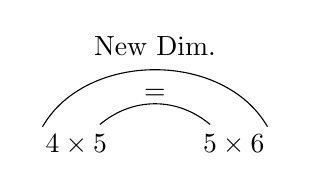
\begin{tikzpicture}
	\node at (-1,0) (A) {$4 \times 5$};
	\node at (1,0) (B) {$5 \times 6$};
	\node at (-1.5,0.1) (Ap) {};
	\node at (1.5,0.1) (Bp) {};
	\draw[bend left=40] (A) to (B) node[midway,above,yshift=0.45cm] {=};
	\draw[bend left=60] (Ap) to (Bp) node[midway,above,yshift=1.0cm] {\text{New Dim.}};
	\end{tikzpicture}
	\]
The matrix $BC$ will have size $4 \times 6$, i.e. 4 rows and 6 columns.} \par\vspace{1.5cm}

\item[(d)] Without explicitly computing $BC$, find the $(3,2)$-entry of the product, i.e. $(BC)_{32}$. \par\vspace{0.3cm}
\wsol{%
	\[
	\begin{aligned}
	(BC)_{32}&= \text{row 3 of } B \cdot \text{column 2 of } C \\[0.2cm]
	&= \langle 1, -2, 1, 0, 2 \rangle \cdot \langle 4, 3, 6, 1, 0 \rangle \\[0.2cm]
	&= 1(4) + (-2) 3 + 1(6) + 0(1) + 2(0) \\[0.2cm]
	&= 4 - 6 + 6 + 0 + 0 \\[0.2cm]
	&= \boxed{4}
	\end{aligned}
	\]%
} \par\vspace{4cm}

\item[(e)] Circle the pivot positions in $D$ and determine its rank and nullity. \par\vspace{0.3cm}
\wsol{Observe $D$ is in RREF. There are three pivot positions. So, $D$ has rank 3. But then $D$ has nullity $\# \text{ col} - \text{rank}= 5 - 3= 2$.
	\[
	\boxed{%
	\begin{gathered}
	\text{rank } D= 3 \\
	\text{nullity } D= 2
	\end{gathered}}
	\]%
}
\end{enumerate}



% Question 
\newpage
\question[15] Suppose an augmented matrix $[A \;\mathbf{b}]$ coming from a linear system of equations was placed into REF using the following row operations: \par
	\begin{table}[!ht]
	\centering
	\begin{tabular}{c}
	$R_1 \longleftrightarrow R_3$ \\[0.1cm]
	$-R_1 + 2R_2 \to R_2$ \\[0.1cm]
	$R_1 + R_3 \to R_3$ \\[0.1cm]
	$\frac{1}{3} R_2 \to R_2$ \\[0.1cm]
	$R_2 - R_3 \to R_3$
	\end{tabular}
	\end{table} \par
After these row operations, the following augmented matrix was obtained:
%	\[
%	\left[
%	\begin{array}{ccc|c}
%	1 & 1 & -1 & 4 \\
%	0 & 2 & 3 & 1 \\
%	0 & 0 & 3 & -3
%	\end{array}
%	\right]
%	\]

	\[
	\left[
	\begin{array}{ccc:c} % Uses arydshln
	1 & 1 & -1 & 4 \\
	0 & 2 & 3 & 4 \\
	0 & 0 & 2 & -4
	\end{array}
	\right]
	\]
	
\begin{parts}
\part Labeling your variables $x_1, x_2, \ldots$, find the solution to the original system of linear equations using back-substitution. \par\vspace{0.2cm}
\wsol{%
	\[
	\begin{gathered}
	[0\;0\;2 \;| -\!4] \;\longrightarrow\; 2x_3= -4 \;\longrightarrow\; x_3= -2 \\[0.3cm]
	[0\;2\;3 \;| 1] \;\longrightarrow\; 2x_2 + 3x_3= 4 \;\longrightarrow\; 2x_2 + 3(-2)= 4 \;\longrightarrow\; x_2= 5 \\[0.3cm]
	[1\;1\;-1 \;| 4] \;\longrightarrow\; x_1 + x_2 - x_3= 4 \;\longrightarrow\; x_1 + 5 - (-2)= 4 \;\longrightarrow\; x_1= -3
	\end{gathered}
	\]
	\[
	\boxed{(x_1, x_2, x_3) = (-3, 5, -2)}
	\]
} \vfill

\part Compute the determinant of the original coefficient matrix $A$. \par\vspace{0.3cm}
\wsol{%
We track the changes to the determinant of $A$ as we make the row operations (we label the $i$th matrix in the row reduction $A_i$):
	\begin{table}[!ht]
	\centering
	\begin{tabular}{ccr}
	\wsol{$R_1 \longleftrightarrow R_3$} & \wsol{$\colon$} & \wsol{$\det A= -1 \cdot \det A_1$} \\[0.1cm]
	\wsol{$-R_1 + 2R_2 \to R_2$} & \wsol{$\colon$} & \wsol{$\det A= \tfrac{1}{2} \cdot -1 \cdot \det A_2$} \\[0.1cm]
	\wsol{$R_1 + R_3 \to R_3$} & \wsol{$\colon$} & \wsol{$\det A= \tfrac{1}{2} \cdot -1 \cdot \det A_3$} \\[0.1cm]
	\wsol{$\frac{1}{3} R_2 \to R_2$} & \wsol{$\colon$} & \wsol{$\det A= 3 \cdot \tfrac{1}{2} \cdot -1 \cdot \det A_4$} \\[0.1cm]
	\wsol{$R_2 - R_3 \to R_3$} & \wsol{$\colon$} & \wsol{$\det A= -1 \cdot 3 \cdot \tfrac{1}{2} \cdot -1 \cdot \det A_5$}
	\end{tabular}
	\end{table}
But the matrix $A_5$ is the upper triangular matrix on the left in the given augmented matrix. We know the determinant of an upper triangular matrix is the product of the diagonals. Therefore, we have\dots
	\[
	\det A= -1 \cdot 3 \cdot \tfrac{1}{2} \cdot -1 \cdot \det A_5= -1 \cdot 3 \cdot \tfrac{1}{2} \cdot -1 \cdot \left(1 \cdot 2 \cdot 2 \right)= \boxed{6}
	\]
}
\end{parts}

% Question 
\newpage
\question[15] Matrices $M, N$ below are in RREF and represent augmented matrices coming from systems of linear equations. For each matrix, determine whether the corresponding system is consistent or inconsistent. If it is inconsistent, explain why. If it is consistent, either find the unique solution or parametrize the solution set (if infinitely many solutions exist). Use variables $x_1, x_2, \ldots$\ . 
	\[
	M= \begin{pmatrix} 1 & 0 & 0 & 0 & 0 & 5 \\ 0 & 1 & 0 & 0 & 0 & -2 \\ 0 & 0 & 1 & 0 & 0 & 1 \\ 0 & 0 & 0 & 1 & 0 & 3 \\ 0 & 0 & 0 & 0 & 1 & 0 \\ 0 & 0 & 0 & 0 & 0 & 0 \end{pmatrix}, \qquad
	N= 
	\begin{pmatrix}
	1 & 0 & 0 & 0 & 0 \\
	0 & 1 & 0 & 0 & 0 \\
	0 & 0 & 1 & 0 & 0 \\
	0 & 0 & 0 & 1 & 0 \\
	0 & 0 & 0 & 0 & 1
	\end{pmatrix}
	\] \par\vspace{0.2cm}

\begin{parts}
\part The System Corresponding to $M$: \par\vspace{0.3cm}
\wsol{The system is consistent. We have no row corresponding to $0= \text{ nonzero number}$. Recalling that the columns correspond to $x_1, x_2, \ldots$, respectively, writing down each equation gives the following unique solution.
	\[
	\begin{cases}
	x_1= 5 \\
	x_2= -2 \\
	x_3= 1 \\
	x_4= 3 \\
	x_5= 0
	\end{cases}
	\]%
} \par\vspace{2.5cm}

\part The System Corresponding to $N$: \par\vspace{0.3cm}
\wsol{Observe that the last row corresponds to an equation $0= 1$, which is a contradiction. Therefore, the corresponding system of linear equations has no solution. So, the system is inconsistent.}
\end{parts}


% Question 
\newpage
\question[15] A system of linear equations with infinitely many solutions has an augmented matrix whose RREF form is given below.
	\[
	\begin{bmatrix}
	1 & 0 & -1 & 0 & 3 \\
	0 & 1 & 2 & -1 & 5 \\
	0 & 0 & 0 & 0 & 0 
	\end{bmatrix}
	\]
Find all of the possible solutions in vector form. Label the variables $x_1, x_2, \ldots$\ . Also, give a concrete example of one of the infinitely many possible solutions. \par\vspace{0.3cm}

\vsol{\itshape We emphasize the fact that this is an augmented matrix.
	\[
	\left[
	\begin{array}{cccc:c}
	\boxed{1} & 0 & -1 & 0 & 3 \\
	0 & \boxed{1} & 2 & -1 & 5 \\
	0 & 0 & 0 & 0 & 0 
	\end{array}
	\right]
	\]
We know the first four columns correspond to $x_1, x_2, x_3, x_4$, respectively. Because the first two columns have a pivot position (boxed), these are pivot columns so $x_1, x_2$ are basic variables. Therefore, $x_3$ and $x_4$ are free variables. Let us write $x_3= a$ and $x_4= b$, where $a, b$ are arbitrary real numbers. Writing the equations corresponding to the first two rows (the last simply states $0= 0$), we have\dots
	\[
	\begin{gathered}
	x_1 - x_3= 3 \\
	x_2 + 2x_3 - x_4= 5
	\end{gathered}
	\]
Therefore, we know that $x_1= x_3 + 3= a + 3$ and $x_2= -2x_3 + x_4 + 5= -2a + b + 5$. So, we have\dots
	\[
	\begin{pmatrix} x_1 \\ x_2 \\ x_3 \\ x_4 \end{pmatrix}= \begin{pmatrix} a + 3 \\ -2a + b + 5 \\ a \\ b \end{pmatrix}= \begin{pmatrix} 3 \\ 5 \\ 0 \\ 0 \end{pmatrix} + \begin{pmatrix} a \\ -2a \\ a \\ 0 \end{pmatrix} + \begin{pmatrix} 0 \\ b \\ 0 \\ b \end{pmatrix}= \boxed{\begin{pmatrix} 3 \\ 5 \\ 0 \\ 0 \end{pmatrix} + a \begin{pmatrix} 1 \\ -2 \\ 1 \\ 0 \end{pmatrix} + b \begin{pmatrix} 0 \\ 1 \\ 0 \\ 1 \end{pmatrix}}
	\]
We may choose any real numbers $a, b$ to find a particular solution. For instance, \dots
	\[
	\begin{aligned}
	a=b=0 \colon& \begin{pmatrix} 3 \\ 5 \\ 0 \\ 0 \end{pmatrix} + 0 \begin{pmatrix} 1 \\ -2 \\ 1 \\ 0 \end{pmatrix} + 0 \begin{pmatrix} 0 \\ 1 \\ 0 \\ 1 \end{pmatrix}= \begin{pmatrix} 3 \\ 5 \\ 0 \\ 0 \end{pmatrix} \\[0.2cm]
	a=1, b=0 \colon& \begin{pmatrix} 3 \\ 5 \\ 0 \\ 0 \end{pmatrix} + 1 \begin{pmatrix} 1 \\ -2 \\ 1 \\ 0 \end{pmatrix} + 0 \begin{pmatrix} 0 \\ 1 \\ 0 \\ 1 \end{pmatrix}= \begin{pmatrix} 4 \\ 3 \\ 1 \\ 0 \end{pmatrix} \\[0.2cm]
	a=0, b=1 \colon& \begin{pmatrix} 3 \\ 5 \\ 0 \\ 0 \end{pmatrix} + 0 \begin{pmatrix} 1 \\ -2 \\ 1 \\ 0 \end{pmatrix} + 1 \begin{pmatrix} 0 \\ 1 \\ 0 \\ 1 \end{pmatrix}= \begin{pmatrix} 3 \\ 6 \\ 0 \\ 1 \end{pmatrix}
	\end{aligned}
	\]
}

\end{questions}
\end{document}